\label{compileandrun}
This chapter explain the POP-Java compilation process, the POP-Java application launching process and the tools related to those processes. The structure of this chapter is as follows : The first section explains the compilation process and the special compiler for POP-Java. The second describes the application launching tools. The third one aims to help the programmer to understand the importance of the object map and the object map generator in the POP-Java application launching process. Finally, a full example is explained to pass trough the whole process. 


\subsection{The POP-Java compiler}
POP-Java has its own compilation process. As POP-Java applications are written in the POP-Java language, the programmer have to use the POP-Java compiler to compile its application. The figure [\ref{fig:popjava_compiler}] shows the POP-Java compilation process. The POP-Java source files will be converted in standard Java source files by a specific parser and code generator. These Java source files will be compiled with the POP-Java library and produce compiled class files or a Java archive file (JAR). \s


\begin{figure}[ht]
	\caption{POP-Java compilation process}
  	\centering
	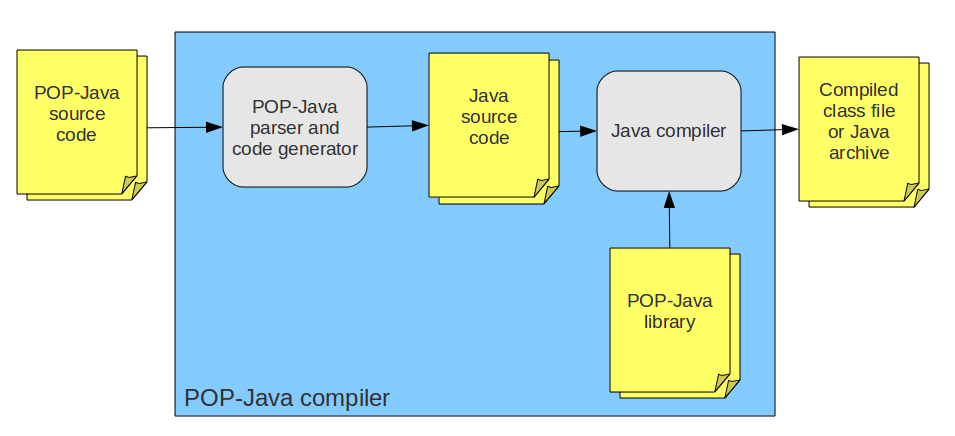
\includegraphics[scale=0.6]{popjcompiler.png}
	\label{fig:popjava_compiler}
\end{figure}

The POP-Java compiler will parse and generate new source file only for the files with .pjava extension. Due to that, it is very important the main class and the parallel classes have this extension and not the standard .java extension.\s

The POP-Java compiler is accessible trough the command "popjc". The command syntax is as follow : 
\begin{lstlisting}
popjc <options> <files>
\end{lstlisting}\s

Options
\begin{itemize}
\item -n or --noclean : Do not clean the temporary files generated by the parser and code generator. 
\item -p or --popcpp : Use the specified additional informations XML file for the compilation (See chapter \ref{mixed}).
\item -j or --jar : Compile the source files in a JAR file. Name of the JAR must be specified.
\item -v or --verbose : Print additional information during the compilation process. 
\item -c or --classpath : Add class file or JAR file to the compilation
\item -x or --xmlpopcpp : Generate the XML additional information file with the specified source files (See chapter \ref{mixed}).
\item -g or --generate : Generate the POP-C++ partial implementation from the specified source file (See chapter \ref{mixed}). Not implemented in the current version.
\end{itemize}

The files in the command line are the ones to compile (.pjava or .java). The command help is available in the appendix \ref{popjc_help}.


\subsection{The POP-Java application launcher}
To help POP-Java programmer, POP-Java provide an application launcher that simplify the launch of a POP-Java application. This application launcher is named "popjrun" and is used with the following syntax : 

\begin{lstlisting}
popjrun <options> [<objectmap>] <MainClass> <arguments>
\end{lstlisting}\s

Here is an explanation of the arguments to provide to the POP-Java application launcher : 

\begin{itemize}
\item \textbf{options} : in the current version there is only one option "-c" or "--classpath" that allow the programmer to add some class path for the execution of the POP-Java application. The different class paths must be separated with a semicolon.
\item \textbf{objectmap} : this informations is not mandatory. If it's provided, the object map inform the runtime system about the location of the different compiled parallel classes of the application. If it's not provided, the default object map (located under : \textit{POPJAVA\_LOCATION}/etc/defaultobjectmap.xml) will be used. More information give in the section \ref{objectmap}.
\item \textbf{MainClass} : this is a main class of the POP-Java application.
\item \textbf{arguments} : there are the arguments of the program
\end{itemize}


\subsection{The POP-Java object map and object map generator}
\label{objectmap}
The object map is an XML file that informs the POP-C++ runtime about the location of the different compiled parallel classes of the application. This file can be given to the "popjrun" tool. If the programmer do not give this file, the default object map located in \textit{POPJAVA\_LOCATION}/etc/ will be used. \s

The object map can be generated with the POP-Java application launcher. By using the option "-l" or "--listlong" and giving the class files or the JAR file, the object map will be printed to the standard output. The easiest way to save this file is to redirect the output into the desired file.\s

Here are the command used for our example : \s

\textbf{Compiled classes}
\begin{lstlisting}
popjrun --listlong Parclass1.class:Parclass2.class > objectmap.xml
\end{lstlisting}\s

\textbf{JAR file}
\begin{lstlisting}
popjrun --listlong parclasses.jar > objectmap.xml
\end{lstlisting}

\pagebreak
\subsection{Full example}
This section shows how to write, compile and launch a POP-Java application by using a simple example. The POP-Java application used in this example includes only one parallel class. All sources of this example can be found in the directory "examples/integer" from the POP-Java distribution.

\subsubsection{Programming}
When we start to develop a POP-Java application the main part is the parallel classes. The figure [\ref{fig:code_integer.pjava}] shows the parallel class implementation. As we can see this class use special POP-Java keywords. In the line 1, the parclass keyword specifies that this class is a parallel class. The constructor declaration includes an object description (line 4). The method declarations includes the invocation semantics (line 8, 12 and 16). The method "add" (line 16) receive another parallel object as a parameter and it's transparent for the programmer.

\begin{figure}[ht]
\caption{File Integer.pjava}
\label{fig:code_integer.pjava}
\begin{lstlisting}
1:  @POPClass
2:  public class Integer {
3:    private int value;
4:	
5:        @POPObjectDescription(url="localhost")
6:	  public Integer(){
7:	    value = 0;	
8: 	  }
9: 	
10:	  @POPSyncConc
11:	  public int get(){
12:	    return value	
13:	  }
14:	
15:	  @POPAsyncSeq
16:	  public void set(int val){
17:	    value = val;	
18:	  }
19:	
20:       @POPAsyncMutex
21:	  public void add(Integer i){
22:	    value += i.get();	
23:	  }
24:	}
\end{lstlisting}
\end{figure}

\pagebreak
Once the parallel class is implemented, we can write a main class that use this parallel class.
The figure [\ref{fig:code_testinteger.pjava}] shows the code of the main class. The code of the main class is pure Java code.
However, this code must be declared in a file with ".pjava" extension to be considered by the POP-Java compiler.
The instantiation (lines 3-4) and the method calls (lines 5-9) are transparent for the programmer.

\begin{figure}[ht]
\caption{File TestInteger.pjava}
\label{fig:code_testinteger.pjava}
\begin{lstlisting}
1: 	public TestInteger {
2: 	  public static void main(String[] args){
3:	    Integer i1 = new Integer();
4:	    Integer i2 = new Integer();
5:	    i1.set(23);
6:	    i2.set(25);
7:	    System.out.println("i1=" + i1.get());
8:	    System.out.println("i2=" + i2.get());
9:	    i1.add(i2);
10:	    int sum =  i1.get();
11:	    System.out.println("i1+i2 = "+sum);
12:	    if(sum==48)
13:	      System.out.println("Test Integer Successful");
14:	    else
15:	      System.out.println("Test Integer failed");
16:	    }
17:	}
\end{lstlisting}
\end{figure}


\subsubsection{Compiling}
The POP-Java compiler can generate two kind of compiled code. The first is the standard Java compiled class file (.class). The second is the Java archive (JAR) file. Here are the two commands to compile the example application.\s

\textbf{Compiling as .class files}
\begin{lstlisting}
popjc Integer.pjava TestInteger.pjava
\end{lstlisting}\s

\textbf{Compiling as a JAR file}
\begin{lstlisting}
popjc -j myjar.jar Integer.pjava TestInteger.pjava
\end{lstlisting}

\subsubsection{Create the object map}
Before running the example application, the programmer needs to generate the object map. The object map will be given to the POP-Java launcher. This file will inform the POP-C++ runtime system where to find the compiled files. The POP-Java launcher has a specific option to generate this file from the compiled files (.class) or the JAR file (.jar). Here is the command used for our example :

\begin{lstlisting}
popjrun --listlong Integer.class > objmap.xml
\end{lstlisting}\s

The command will generate the XML file and print it on the standard output. To save this file, we redirect the output in a file named objmap.xml. This file contains the following XML code (the path specified in the element CodeFile will be different on your computer) : 

\begin{lstlisting}
<CodeInfoList>
  <CodeInfo>
    <ObjectName>Integer</ObjectName>
    <CodeFile Type="popjava">
      /home/clementval/pop/popjava-1.0/example/integer/</CodeFile>
    <PlatForm>*-*</PlatForm>
  </CodeInfo>
</CodeInfoList>
\end{lstlisting}


\subsubsection{Running}
Once the POP-Java application is compiled and the object map is generated, the application can be run. A POP-Java application is a pure Java application at the end and could be run with the standard java program. In order to make this running easier for the programmer, POP-Java include an application launcher. Here are the command to use to run the POP-Java application example : \s

\textbf{POP-Java application compiled as .class files}
\begin{lstlisting}
popjrun objectmap.xml TestInteger
\end{lstlisting}\s

\textbf{POP-Java application compiled as .jar file}
\begin{lstlisting}
popjrun -c myjar.jar objectmap.xml TestInteger
\end{lstlisting}\s

\textbf{Application output}\\
Here is what we should have as the application output : 
\begin{lstlisting}
i1=23
i2=25
i1+i2=48
Test Integer Successful 
\end{lstlisting}\s

If we have any problems with the compilation or the launching of the application, please see the chapter \ref{trouble}.
